\chapter{Analysis Details}

We published a paper recently~\cite{SUSY} in which we conducted searches using two classes of SUSY models, denoted the strong and electroweak models. Both types of search looked for final products with two opposite-sign same-flavor leptons, at least two jets, and large \MET. These searches used the full ATLAS Run 2 dataset of $\sqrt{s}$ = 13 TeV collision data, with an integrated luminosity of $139 fb^{-1}$. I participated mostly in the strong search, so this is what I will describe here. Some parts of this section have been taken with changes from the paper.

\section{Signal Models}

We looked at three different models in the strong analysis (Figure~\ref{fig:SUSY_models}), which we called gluino-slepton, gluino-$Z^{(*)}$, and squark-$Z^{(*)}$. In these models, we have pair production of hypothesized SUSY particles (either gluino pairs or squark pairs) which decay in certain ways. There are various floating parameters, such as the masses of the SUSY particles, which are partially scanned over in our signal model production grid.

\begin{figure}[htbp]
    \centering
    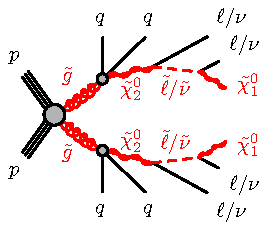
\includegraphics[width=0.32\textwidth]{Images/SUSY/gogo-qqqqllllN1N1-N2.pdf}
    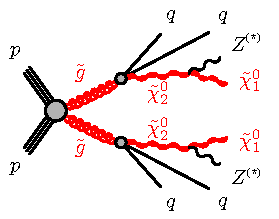
\includegraphics[width=0.32\textwidth]{Images/SUSY/gogo-qqqqZZN1N1.pdf}
    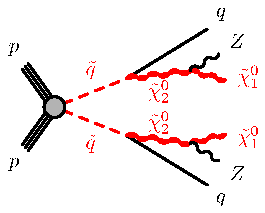
\includegraphics[width=0.32\textwidth]{Images/SUSY/sqsq-qqZZN1N1.pdf}
    \caption{(Left) gluino-slepton model, $\tilde{g}\to qq \tilde{\chi}_2^0$, with $\tilde{\chi}_{2}^{0} \to \tilde{\ell}^{\mp}\ell^{\pm} / \tilde{\nu}\nu$ and $\tilde{\ell}/\tilde{\nu} \to (\ell/\nu)\tilde{\chi}_{1}^{0}$. (Middle) gluino-$Z^{(*)}$ model, $\tilde{g}\to qq \tilde{\chi}_2^0$, with $\tilde{\chi}_2^0\rightarrow Z^{(*)} \tilde{\chi}_1^0$. (Right) squark-$Z^{(*)}$ model, $\tilde{q}\to q \tilde{\chi}_2^0$, with $\tilde{\chi}_2^0\rightarrow Z \tilde{\chi}_1^0$.}
    \label{fig:SUSY_models}
\end{figure}

Each of these models begins with a gluino or squark decaying via quark jets into the second lightest neutralino. These neutralinos then undergo either a two-lepton decay, an on-shell Z decay, or an off-shell Z decay, and end up producing the lightest neutralino, which exits the detector without being detected. Depending on the model, the resulting lepton pairs have different \mll\ distributions. The lightest neutralino, which is also the lightest SUSY particle (LSP) in these models, shows up in our events as \MET.

\section{Signal Production Grids}

In all three models, we consider quark decay or production using five flavors ($u$, $d$, $c$, $s$, $b$) of equal probability. In these simplified models, we ignore all SUSY particles not directly involved in the decay chains, thus considering them to have coupling constants of zero.

As mentioned, the masses of these particles are still unconstrained, so we generate samples in grids over two dimensions, scanning over the LSP mass and either the gluino or squark mass. All squarks are assumed to be mass degenerate in these models. In each case, $\tilde{\chi}_0^2$ is constrained to have a mass halfway between the LSP mass and the mass of the gluino or squark. For example, for the gluino models, $m(\tilde{\chi}_0^2) = [m(\tilde{g})+m(\tilde{\chi^1_0})]/2$. For the slepton model, the masses of the left-handed sleptons are set to $m(\tilde{\ell}) = [m(\tilde{\chi^2_0})+m(\tilde{\chi^1_0})]/2$, while the right-handed sleptons are decoupled.

When the mass difference between $\tilde{\chi}_{2}^{0}$ and $\tilde{\chi}_{1}^{0}$ is less than the $Z$ mass, we have an off-shell model. Otherwise we have an on-Z signal.

The signal samples are produced using MadGraph5 with the NNPDF LO PDF set and contain up to one additional parton in the matrix element. The generation uses Pythia8 for showering and hadronization with EvtGen and the ATLAS A14 tune and the CTEQ 6L1 PDF set in the shower. Decoupled sparticles are vetoed in the production diagrams in MadGraph5. Signal production cross sections are calculated at NNLO$_\text{approx}$ with NNLL resummation. The details of strong signal model generation can be found in the following JIRA tickets~\cite{JIRAGluinoSLN, JIRAGluinoZ, JIRASleptonZ}.

%%%%%%%%%%%%%%%%%%%%%%%%%%%%%

\section{Physics Objects}

When selecting objects for this analysis, we decided to use signal leptons with transverse momentum ($p_T$) above 25 GeV, and jets with $p_T$ above 30 GeV. For the purposes of performing jet overlap removal and calculating $E_T^{miss}$, we also allowed baseline leptons above 10 GeV and baseline jets above 20 GeV. In the interest of keeping this paper at a reasonable length, the complete set of object selection and triggering criteria will not be included, but can be found in the complete SUSY analysis paper at \cite{SUSY_2l2j}.

As with most high-energy physics searches, there were a variety of standard-model processes which mimicked the final state we were looking for. Of these, the $t\bar{t}$ process was the largest, followed by diboson (WZ/ZZ) processes. Events with a single Z and two or more jets from initial-state radiation could also mimic our signal, provided that mismeasurement of the jet momentum resulted in a large $E_T^{miss}$ for the event. Events from single-top-quark processes and from lepton misidentification also contributed to the background. To accurately model these backgrounds, we used flavor-symmetry, Z/$\gamma^*$, Monte Carlo, and fake estimation methods, all of which will be described below.

As we had several unknown masses in our models, we needed to find multiple signal regions which could optimize the signal-to-background ratio for a variety of different $\tilde{\chi}^0_1$, $\tilde{\chi}^0_2$, and $\tilde{g}$ masses. In Figure~\ref{signal_regions}, we show the four signal regions we chose, along with their associated validation and control regions, which were used to implement and test various background-rejection methods.

\section{Regions}